\documentclass[twoside]{book}

% Packages required by doxygen
\usepackage{calc}
\usepackage{doxygen}
\usepackage{graphicx}
\usepackage[utf8]{inputenc}
\usepackage{makeidx}
\usepackage{multicol}
\usepackage{multirow}
\usepackage{textcomp}
\usepackage[table]{xcolor}

% Font selection
\usepackage[T1]{fontenc}
\usepackage{mathptmx}
\usepackage[scaled=.90]{helvet}
\usepackage{courier}
\usepackage{amssymb}
\usepackage{sectsty}
\renewcommand{\familydefault}{\sfdefault}
\allsectionsfont{%
  \fontseries{bc}\selectfont%
  \color{darkgray}%
}
\renewcommand{\DoxyLabelFont}{%
  \fontseries{bc}\selectfont%
  \color{darkgray}%
}

% Page & text layout
\usepackage{geometry}
\geometry{%
  a4paper,%
  top=2.5cm,%
  bottom=2.5cm,%
  left=2.5cm,%
  right=2.5cm%
}
\tolerance=750
\hfuzz=15pt
\hbadness=750
\setlength{\emergencystretch}{15pt}
\setlength{\parindent}{0cm}
\setlength{\parskip}{0.2cm}
\makeatletter
\renewcommand{\paragraph}{%
  \@startsection{paragraph}{4}{0ex}{-1.0ex}{1.0ex}{%
    \normalfont\normalsize\bfseries\SS@parafont%
  }%
}
\renewcommand{\subparagraph}{%
  \@startsection{subparagraph}{5}{0ex}{-1.0ex}{1.0ex}{%
    \normalfont\normalsize\bfseries\SS@subparafont%
  }%
}
\makeatother

% Headers & footers
\usepackage{fancyhdr}
\pagestyle{fancyplain}
\fancyhead[LE]{\fancyplain{}{\bfseries\thepage}}
\fancyhead[CE]{\fancyplain{}{}}
\fancyhead[RE]{\fancyplain{}{\bfseries\leftmark}}
\fancyhead[LO]{\fancyplain{}{\bfseries\rightmark}}
\fancyhead[CO]{\fancyplain{}{}}
\fancyhead[RO]{\fancyplain{}{\bfseries\thepage}}
\fancyfoot[LE]{\fancyplain{}{}}
\fancyfoot[CE]{\fancyplain{}{}}
\fancyfoot[RE]{\fancyplain{}{\bfseries\scriptsize Generated on Thu Dec 10 2015 20\-:39\-:50 for A\-F\-\_\-\-H\-F by Doxygen }}
\fancyfoot[LO]{\fancyplain{}{\bfseries\scriptsize Generated on Thu Dec 10 2015 20\-:39\-:50 for A\-F\-\_\-\-H\-F by Doxygen }}
\fancyfoot[CO]{\fancyplain{}{}}
\fancyfoot[RO]{\fancyplain{}{}}
\renewcommand{\footrulewidth}{0.4pt}
\renewcommand{\chaptermark}[1]{%
  \markboth{#1}{}%
}
\renewcommand{\sectionmark}[1]{%
  \markright{\thesection\ #1}%
}

% Indices & bibliography
\usepackage{natbib}
\usepackage[titles]{tocloft}
\setcounter{tocdepth}{3}
\setcounter{secnumdepth}{5}
\makeindex

% Custom commands
\newcommand{\clearemptydoublepage}{%
  \newpage{\pagestyle{empty}\cleardoublepage}%
}


%===== C O N T E N T S =====

\begin{document}

% Titlepage & ToC
\pagenumbering{roman}
\begin{titlepage}
\vspace*{7cm}
\begin{center}%
{\Large A\-F\-\_\-\-H\-F }\\
\vspace*{1cm}
{\large Generated by Doxygen 1.8.6}\\
\vspace*{0.5cm}
{\small Thu Dec 10 2015 20:39:50}\\
\end{center}
\end{titlepage}
\clearemptydoublepage
\tableofcontents
\clearemptydoublepage
\pagenumbering{arabic}

%--- Begin generated contents ---
\chapter{Hierarchical Index}
\section{Class Hierarchy}
This inheritance list is sorted roughly, but not completely, alphabetically\-:\begin{DoxyCompactList}
\item Q\-Object\begin{DoxyCompactList}
\item \contentsline{section}{Application\-Window}{\pageref{class_application_window}}{}
\item \contentsline{section}{Message\-\_\-\-Handler}{\pageref{class_message___handler}}{}
\item \contentsline{section}{Quadro\-\_\-msg}{\pageref{class_quadro__msg}}{}
\end{DoxyCompactList}
\item \contentsline{section}{qt\-\_\-meta\-\_\-stringdata\-\_\-\-Application\-Window\-\_\-t}{\pageref{structqt__meta__stringdata___application_window__t}}{}
\item \contentsline{section}{qt\-\_\-meta\-\_\-stringdata\-\_\-\-Message\-\_\-\-Handler\-\_\-t}{\pageref{structqt__meta__stringdata___message___handler__t}}{}
\item \contentsline{section}{qt\-\_\-meta\-\_\-stringdata\-\_\-\-Quadro\-\_\-msg\-\_\-t}{\pageref{structqt__meta__stringdata___quadro__msg__t}}{}
\item \contentsline{section}{qt\-\_\-meta\-\_\-stringdata\-\_\-\-T\-C\-P\-\_\-com\-\_\-t}{\pageref{structqt__meta__stringdata___t_c_p__com__t}}{}
\item Q\-Thread\begin{DoxyCompactList}
\item \contentsline{section}{T\-C\-P\-\_\-com}{\pageref{class_t_c_p__com}}{}
\end{DoxyCompactList}
\end{DoxyCompactList}

\chapter{Class Index}
\section{Class List}
Here are the classes, structs, unions and interfaces with brief descriptions\-:\begin{DoxyCompactList}
\item\contentsline{section}{{\bf Application\-Window} }{\pageref{class_application_window}}{}
\item\contentsline{section}{{\bf Message\-\_\-\-Handler} }{\pageref{class_message___handler}}{}
\item\contentsline{section}{{\bf qt\-\_\-meta\-\_\-stringdata\-\_\-\-Application\-Window\-\_\-t} }{\pageref{structqt__meta__stringdata___application_window__t}}{}
\item\contentsline{section}{{\bf qt\-\_\-meta\-\_\-stringdata\-\_\-\-Message\-\_\-\-Handler\-\_\-t} }{\pageref{structqt__meta__stringdata___message___handler__t}}{}
\item\contentsline{section}{{\bf qt\-\_\-meta\-\_\-stringdata\-\_\-\-Quadro\-\_\-msg\-\_\-t} }{\pageref{structqt__meta__stringdata___quadro__msg__t}}{}
\item\contentsline{section}{{\bf qt\-\_\-meta\-\_\-stringdata\-\_\-\-T\-C\-P\-\_\-com\-\_\-t} }{\pageref{structqt__meta__stringdata___t_c_p__com__t}}{}
\item\contentsline{section}{{\bf Quadro\-\_\-msg} \\*A robot szimulátor üzenet }{\pageref{class_quadro__msg}}{}
\item\contentsline{section}{{\bf T\-C\-P\-\_\-com} \\*Üzenet feldolgozó }{\pageref{class_t_c_p__com}}{}
\end{DoxyCompactList}

\chapter{Class Documentation}
\section{Application\-Window Class Reference}
\label{class_application_window}\index{Application\-Window@{Application\-Window}}
Inheritance diagram for Application\-Window\-:\begin{figure}[H]
\begin{center}
\leavevmode
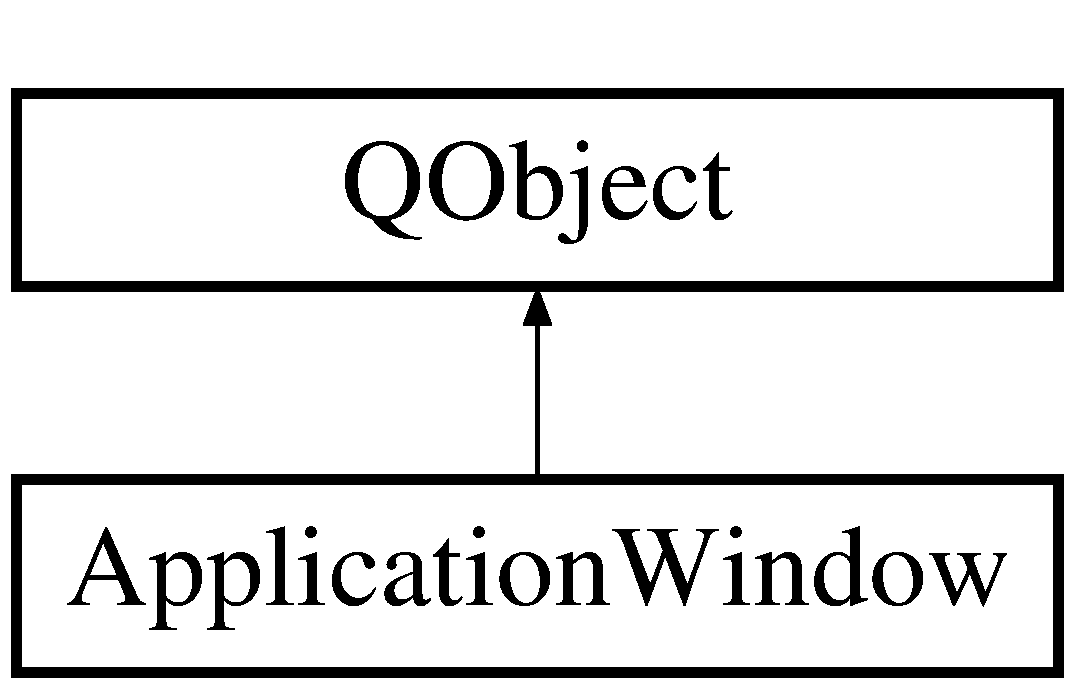
\includegraphics[height=2.000000cm]{class_application_window}
\end{center}
\end{figure}
\subsection*{Public Slots}
\begin{DoxyCompactItemize}
\item 
void {\bfseries Power\-Switch\-Command} ()\label{class_application_window_abc35b58c8ca2c39bd7a298103adfece1}

\item 
void {\bfseries Set\-P\-I\-D\-Command} ()\label{class_application_window_a4a0e87dea2ff1924c5dbcbeac592a214}

\item 
void {\bfseries Refresh\-P\-I\-D\-Command} ()\label{class_application_window_af900f0e296766b3691543f6d4883e9c7}

\item 
void {\bfseries State\-Changed} ()\label{class_application_window_a810fbc32edfda877bf65dc2c48c9f5a4}

\item 
void {\bfseries Get\-State} ({\bf Quadro\-\_\-msg} msg)\label{class_application_window_a9c777b3c7287e46df9d7983cc941b2ea}

\end{DoxyCompactItemize}
\subsection*{Signals}
\begin{DoxyCompactItemize}
\item 
void {\bfseries Context\-Changed} ()\label{class_application_window_a68c39d9258449139a831f5a9349648ad}

\item 
void {\bfseries T\-C\-P\-\_\-send} (Q\-String msg)\label{class_application_window_a7ebea099dd91d7ba1b5d207dfdd8c0fb}

\end{DoxyCompactItemize}
\subsection*{Public Member Functions}
\begin{DoxyCompactItemize}
\item 
{\bfseries Application\-Window} (Q\-Object $\ast$root\-Object, Q\-Qml\-Context \&qml\-Context)\label{class_application_window_a9ed3a7e865a416a3e414fd19d67e69bb}

\item 
void {\bfseries connect\-Qml\-Signals} (Q\-Object $\ast$root\-Object)\label{class_application_window_a8763dd7b8c8a313b98a3ed06ddab0748}

\end{DoxyCompactItemize}


The documentation for this class was generated from the following files\-:\begin{DoxyCompactItemize}
\item 
applicationwindow.\-h\item 
applicationwindow.\-cpp\item 
moc\-\_\-applicationwindow.\-cpp\end{DoxyCompactItemize}

\section{Message\-\_\-\-Handler Class Reference}
\label{class_message___handler}\index{Message\-\_\-\-Handler@{Message\-\_\-\-Handler}}
Inheritance diagram for Message\-\_\-\-Handler\-:\begin{figure}[H]
\begin{center}
\leavevmode
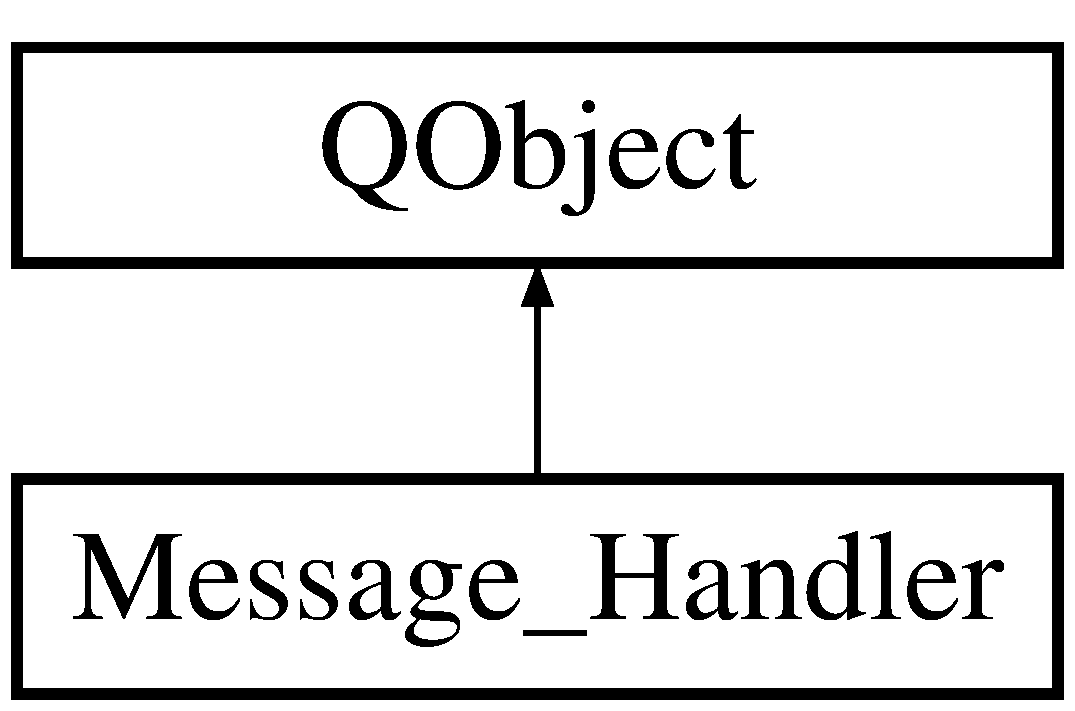
\includegraphics[height=2.000000cm]{class_message___handler}
\end{center}
\end{figure}
\subsection*{Public Member Functions}
\begin{DoxyCompactItemize}
\item 
{\bf Message\-\_\-\-Handler} (Q\-Object $\ast$parent=0)
\item 
void {\bf parser} (Q\-Byte\-Array data)
\begin{DoxyCompactList}\small\item\em Üzenet feldolgozó . \end{DoxyCompactList}\end{DoxyCompactItemize}
\subsection*{Public Attributes}
\begin{DoxyCompactItemize}
\item 
{\bf Quadro\-\_\-msg} {\bfseries msg}\label{class_message___handler_a7a2b3434d1fa11bb5d3a5bf3a0609428}

\end{DoxyCompactItemize}


\subsection{Constructor \& Destructor Documentation}
\index{Message\-\_\-\-Handler@{Message\-\_\-\-Handler}!Message\-\_\-\-Handler@{Message\-\_\-\-Handler}}
\index{Message\-\_\-\-Handler@{Message\-\_\-\-Handler}!Message_Handler@{Message\-\_\-\-Handler}}
\subsubsection[{Message\-\_\-\-Handler}]{\setlength{\rightskip}{0pt plus 5cm}Message\-\_\-\-Handler\-::\-Message\-\_\-\-Handler (
\begin{DoxyParamCaption}
\item[{Q\-Object $\ast$}]{parent = {\ttfamily 0}}
\end{DoxyParamCaption}
)\hspace{0.3cm}{\ttfamily [explicit]}}\label{class_message___handler_aa2b0628ac18ee54e0972a232035e1bb7}
Konstruktor 

\subsection{Member Function Documentation}
\index{Message\-\_\-\-Handler@{Message\-\_\-\-Handler}!parser@{parser}}
\index{parser@{parser}!Message_Handler@{Message\-\_\-\-Handler}}
\subsubsection[{parser}]{\setlength{\rightskip}{0pt plus 5cm}void Message\-\_\-\-Handler\-::parser (
\begin{DoxyParamCaption}
\item[{Q\-Byte\-Array}]{data}
\end{DoxyParamCaption}
)}\label{class_message___handler_accd3fd920264b1b773a05f47668bb08f}


Üzenet feldolgozó . 

J\-S\-O\-N parser 
\begin{DoxyParams}{Parameters}
{\em data} & bejövő J\-S\-O\-N adatcsomag.\\
\hline
\end{DoxyParams}
Bejövő J\-S\-O\-N string-\/et alakítja \doxyref{Quadro\-\_\-msg}{p.}{class_quadro__msg} formáturmra A feldolgozott adatot \doxyref{Quadro\-\_\-msg}{p.}{class_quadro__msg} Objektumba írja 

The documentation for this class was generated from the following files\-:\begin{DoxyCompactItemize}
\item 
message\-\_\-handler.\-h\item 
message\-\_\-handler.\-cpp\end{DoxyCompactItemize}

\section{qt\-\_\-meta\-\_\-stringdata\-\_\-\-Application\-Window\-\_\-t Struct Reference}
\label{structqt__meta__stringdata___application_window__t}\index{qt\-\_\-meta\-\_\-stringdata\-\_\-\-Application\-Window\-\_\-t@{qt\-\_\-meta\-\_\-stringdata\-\_\-\-Application\-Window\-\_\-t}}
\subsection*{Public Attributes}
\begin{DoxyCompactItemize}
\item 
Q\-Byte\-Array\-Data {\bfseries data} [11]\label{structqt__meta__stringdata___application_window__t_a50cb6669db072d15204e3a28d6a6b42b}

\item 
char {\bfseries stringdata} [132]\label{structqt__meta__stringdata___application_window__t_a1462c5c87e5eb4ceb8d2a85507f23a30}

\end{DoxyCompactItemize}


The documentation for this struct was generated from the following file\-:\begin{DoxyCompactItemize}
\item 
moc\-\_\-applicationwindow.\-cpp\end{DoxyCompactItemize}

\section{qt\-\_\-meta\-\_\-stringdata\-\_\-\-Message\-\_\-\-Handler\-\_\-t Struct Reference}
\label{structqt__meta__stringdata___message___handler__t}\index{qt\-\_\-meta\-\_\-stringdata\-\_\-\-Message\-\_\-\-Handler\-\_\-t@{qt\-\_\-meta\-\_\-stringdata\-\_\-\-Message\-\_\-\-Handler\-\_\-t}}
\subsection*{Public Attributes}
\begin{DoxyCompactItemize}
\item 
Q\-Byte\-Array\-Data {\bfseries data} [9]\label{structqt__meta__stringdata___message___handler__t_ac71c3bf20872ed0a82a95e157143d8ee}

\item 
char {\bfseries stringdata} [117]\label{structqt__meta__stringdata___message___handler__t_a9f65437ee106bdf2d3a61ac1f7dbfd12}

\end{DoxyCompactItemize}


The documentation for this struct was generated from the following file\-:\begin{DoxyCompactItemize}
\item 
moc\-\_\-message\-\_\-handler.\-cpp\end{DoxyCompactItemize}

\section{qt\-\_\-meta\-\_\-stringdata\-\_\-\-Quadro\-\_\-msg\-\_\-t Struct Reference}
\label{structqt__meta__stringdata___quadro__msg__t}\index{qt\-\_\-meta\-\_\-stringdata\-\_\-\-Quadro\-\_\-msg\-\_\-t@{qt\-\_\-meta\-\_\-stringdata\-\_\-\-Quadro\-\_\-msg\-\_\-t}}
\subsection*{Public Attributes}
\begin{DoxyCompactItemize}
\item 
Q\-Byte\-Array\-Data {\bfseries data} [1]\label{structqt__meta__stringdata___quadro__msg__t_a64fddaab421047a5fe6034c187a8b02e}

\item 
char {\bfseries stringdata} [12]\label{structqt__meta__stringdata___quadro__msg__t_a9189c2de4834378f59894644f6aaa686}

\end{DoxyCompactItemize}


The documentation for this struct was generated from the following file\-:\begin{DoxyCompactItemize}
\item 
moc\-\_\-quadro\-\_\-msg.\-cpp\end{DoxyCompactItemize}

\section{qt\-\_\-meta\-\_\-stringdata\-\_\-\-T\-C\-P\-\_\-com\-\_\-t Struct Reference}
\label{structqt__meta__stringdata___t_c_p__com__t}\index{qt\-\_\-meta\-\_\-stringdata\-\_\-\-T\-C\-P\-\_\-com\-\_\-t@{qt\-\_\-meta\-\_\-stringdata\-\_\-\-T\-C\-P\-\_\-com\-\_\-t}}
\subsection*{Public Attributes}
\begin{DoxyCompactItemize}
\item 
Q\-Byte\-Array\-Data {\bfseries data} [11]\label{structqt__meta__stringdata___t_c_p__com__t_a7936d3e222d40a3f2cbdc7f70bfe3492}

\item 
char {\bfseries stringdata} [125]\label{structqt__meta__stringdata___t_c_p__com__t_af357223b35d9926d0c10a4f56e285f68}

\end{DoxyCompactItemize}


The documentation for this struct was generated from the following file\-:\begin{DoxyCompactItemize}
\item 
moc\-\_\-tcp\-\_\-com.\-cpp\end{DoxyCompactItemize}

\section{Quadro\-\_\-msg Class Reference}
\label{class_quadro__msg}\index{Quadro\-\_\-msg@{Quadro\-\_\-msg}}


A robot szimulátor üzenet .  




{\ttfamily \#include $<$quadro\-\_\-msg.\-h$>$}

Inheritance diagram for Quadro\-\_\-msg\-:\begin{figure}[H]
\begin{center}
\leavevmode
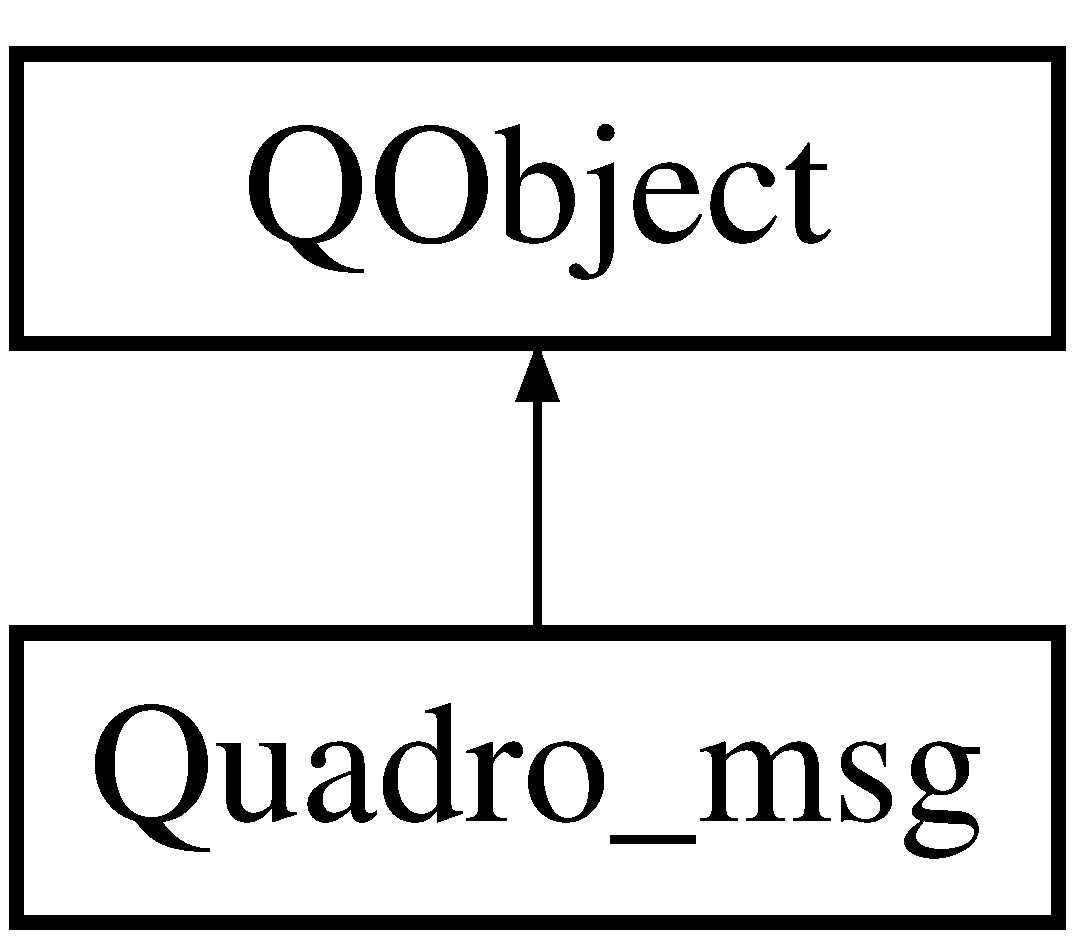
\includegraphics[height=2.000000cm]{class_quadro__msg}
\end{center}
\end{figure}
\subsection*{Public Member Functions}
\begin{DoxyCompactItemize}
\item 
{\bfseries Quadro\-\_\-msg} (Q\-Object $\ast$parent=0)\label{class_quadro__msg_a38b36dc15f77161bcddce4f7975ab043}

\item 
{\bfseries Quadro\-\_\-msg} (const {\bf Quadro\-\_\-msg} \&other)\label{class_quadro__msg_a545277124fe3dee2e66245aa0b60abd4}

\item 
void {\bfseries clear} ()\label{class_quadro__msg_a41ada14c94d10d0a3fa0e50b40c2e24a}

\item 
void {\bfseries out} ()\label{class_quadro__msg_a8f74e212a5b72e132f2bf60d68b33b9a}

\end{DoxyCompactItemize}
\subsection*{Public Attributes}
\begin{DoxyCompactItemize}
\item 
int {\bfseries Message\-Type}\label{class_quadro__msg_ae1339b41d22e734540f5bbe99b9432a8}

\item 
double {\bfseries Kalman\-X}\label{class_quadro__msg_a1cccf8e943ddceb82caf81b2d2f8cd51}

\item 
double {\bfseries Kalman\-Y}\label{class_quadro__msg_ab9b6082204ee9997b4d9f6eb8886b424}

\item 
double {\bfseries Altitude}\label{class_quadro__msg_a300bb6903242c55dc1ca812584ca6b95}

\item 
bool {\bfseries Main\-Power\-Status}\label{class_quadro__msg_a5aef74662f9298834d7ab719ec64c5fe}

\item 
int {\bfseries Motor\-State0}\label{class_quadro__msg_a9c0b682463a2a11f959cf625014762b1}

\item 
int {\bfseries Motor\-State1}\label{class_quadro__msg_a1b69585f25ffc60a31713501217719c2}

\item 
int {\bfseries Motor\-State2}\label{class_quadro__msg_afd82373ac92fe24be8f7a1455d389ad8}

\item 
int {\bfseries Motor\-State3}\label{class_quadro__msg_a3ce4418ab197741b175db47bfa27e0dd}

\item 
int {\bfseries Kp}\label{class_quadro__msg_add35dfbf7b074a79fbfab2fdc5b42d03}

\item 
int {\bfseries Ki}\label{class_quadro__msg_a8e61618ca1ff007a341d735eebca7349}

\item 
int {\bfseries Kd}\label{class_quadro__msg_aaa6bb4ba4b154377519d8ec323907bbf}

\item 
bool {\bfseries Set\-P\-I\-D\-Success}\label{class_quadro__msg_ae467cf9dc29a026ee7baa92b46dcc18f}

\end{DoxyCompactItemize}


\subsection{Detailed Description}
A robot szimulátor üzenet . 

Tartalmazza az összes mezőt, ami az üzenetekben található. A továbbiakban a beérkezett J\-S\-O\-N formátumú üzeneteket a parser egy ilyen objektumba írja Valamint a G\-U\-I és a kommunikációs réteg között az adatok cseréje \char`\"{}ezzel történik\char`\"{} 

The documentation for this class was generated from the following files\-:\begin{DoxyCompactItemize}
\item 
quadro\-\_\-msg.\-h\item 
quadro\-\_\-msg.\-cpp\end{DoxyCompactItemize}

\section{T\-C\-P\-\_\-com Class Reference}
\label{class_t_c_p__com}\index{T\-C\-P\-\_\-com@{T\-C\-P\-\_\-com}}


Üzenet feldolgozó .  




{\ttfamily \#include $<$tcp\-\_\-com.\-h$>$}

Inheritance diagram for T\-C\-P\-\_\-com\-:\begin{figure}[H]
\begin{center}
\leavevmode
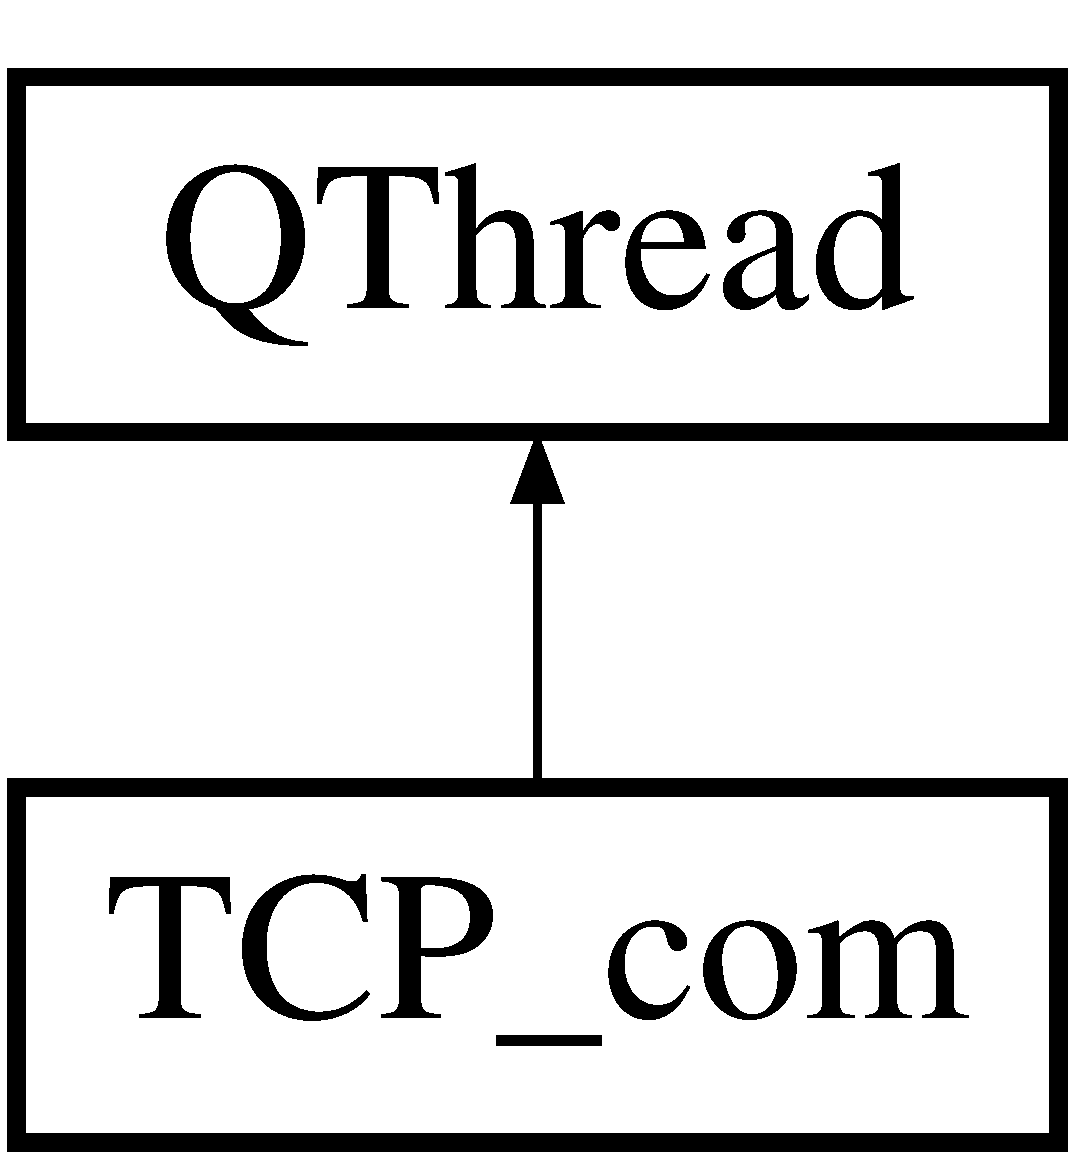
\includegraphics[height=2.000000cm]{class_t_c_p__com}
\end{center}
\end{figure}
\subsection*{Public Slots}
\begin{DoxyCompactItemize}
\item 
void {\bfseries ready\-Read} ()\label{class_t_c_p__com_a4f8efa4eb88ec28e773925ec91802179}

\item 
void {\bf send} (Q\-String command)
\end{DoxyCompactItemize}
\subsection*{Signals}
\begin{DoxyCompactItemize}
\item 
void {\bfseries Get\-\_\-\-State\-\_\-received} ({\bf Quadro\-\_\-msg} msg)\label{class_t_c_p__com_a2864359bfb79b0a98a14b6e0bfb3e762}

\item 
void {\bfseries Get\-\_\-\-P\-I\-D\-\_\-received} ({\bf Quadro\-\_\-msg} msg)\label{class_t_c_p__com_a20a0efd499ac4a97bebeeab5f0dc6d77}

\item 
void {\bfseries Set\-\_\-\-P\-I\-D\-\_\-received} ({\bf Quadro\-\_\-msg} msg)\label{class_t_c_p__com_a0d4aae92cfde9026c687605769aa269e}

\item 
void {\bfseries Set\-\_\-\-Main\-\_\-\-Power\-\_\-received} ({\bf Quadro\-\_\-msg} msg)\label{class_t_c_p__com_a84d13843639703a78ac0c3b2f58c6a3c}

\end{DoxyCompactItemize}
\subsection*{Public Member Functions}
\begin{DoxyCompactItemize}
\item 
{\bf T\-C\-P\-\_\-com} (Q\-Object $\ast$parent=0)
\item 
void {\bf set\-Port} (int port)
\item 
void {\bf set\-Server} (Q\-String server)
\item 
bool {\bf connect\-\_\-to} ()
\item 
bool {\bf disconnect} ()
\item 
void {\bf handler} ({\bf Quadro\-\_\-msg} \&msg)
\end{DoxyCompactItemize}


\subsection{Detailed Description}
Üzenet feldolgozó . 

Kommunikációs csatorna Adatokat feldolgozása \doxyref{Quadro\-\_\-msg}{p.}{class_quadro__msg} objektumba A jelek bekötésével kommuniál a G\-U\-I-\/val 

\subsection{Constructor \& Destructor Documentation}
\index{T\-C\-P\-\_\-com@{T\-C\-P\-\_\-com}!T\-C\-P\-\_\-com@{T\-C\-P\-\_\-com}}
\index{T\-C\-P\-\_\-com@{T\-C\-P\-\_\-com}!TCP_com@{T\-C\-P\-\_\-com}}
\subsubsection[{T\-C\-P\-\_\-com}]{\setlength{\rightskip}{0pt plus 5cm}T\-C\-P\-\_\-com\-::\-T\-C\-P\-\_\-com (
\begin{DoxyParamCaption}
\item[{Q\-Object $\ast$}]{parent = {\ttfamily 0}}
\end{DoxyParamCaption}
)\hspace{0.3cm}{\ttfamily [explicit]}}\label{class_t_c_p__com_a94ce52fa51ee1ed6082b026702907318}
Konstruktor

Konstruktor Message handler és socket létrehozása Socket és a kommunikációs csatorna összekötése 

\subsection{Member Function Documentation}
\index{T\-C\-P\-\_\-com@{T\-C\-P\-\_\-com}!connect\-\_\-to@{connect\-\_\-to}}
\index{connect\-\_\-to@{connect\-\_\-to}!TCP_com@{T\-C\-P\-\_\-com}}
\subsubsection[{connect\-\_\-to}]{\setlength{\rightskip}{0pt plus 5cm}bool T\-C\-P\-\_\-com\-::connect\-\_\-to (
\begin{DoxyParamCaption}
{}
\end{DoxyParamCaption}
)}\label{class_t_c_p__com_aa7a22ac0a393e808da8c4540d44819c4}
T\-C\-P kapcsolódás

Kapcsolódás a szerverhez \index{T\-C\-P\-\_\-com@{T\-C\-P\-\_\-com}!disconnect@{disconnect}}
\index{disconnect@{disconnect}!TCP_com@{T\-C\-P\-\_\-com}}
\subsubsection[{disconnect}]{\setlength{\rightskip}{0pt plus 5cm}bool T\-C\-P\-\_\-com\-::disconnect (
\begin{DoxyParamCaption}
{}
\end{DoxyParamCaption}
)}\label{class_t_c_p__com_ab20ceaf9f60538bbaec5b6e1f4ba322c}
T\-C\-P lekapcsolódás

Kapcsolat lezárása \index{T\-C\-P\-\_\-com@{T\-C\-P\-\_\-com}!handler@{handler}}
\index{handler@{handler}!TCP_com@{T\-C\-P\-\_\-com}}
\subsubsection[{handler}]{\setlength{\rightskip}{0pt plus 5cm}void T\-C\-P\-\_\-com\-::handler (
\begin{DoxyParamCaption}
\item[{{\bf Quadro\-\_\-msg} \&}]{msg}
\end{DoxyParamCaption}
)}\label{class_t_c_p__com_a25497b75e14d2fe6348719aa68d980a5}
üzenetkezelő üzenetekhez megfelelő eventeket generál \index{T\-C\-P\-\_\-com@{T\-C\-P\-\_\-com}!send@{send}}
\index{send@{send}!TCP_com@{T\-C\-P\-\_\-com}}
\subsubsection[{send}]{\setlength{\rightskip}{0pt plus 5cm}void T\-C\-P\-\_\-com\-::send (
\begin{DoxyParamCaption}
\item[{Q\-String}]{msg}
\end{DoxyParamCaption}
)\hspace{0.3cm}{\ttfamily [slot]}}\label{class_t_c_p__com_a2a9af6db5e80f2fb6149341f68918e52}
Adatok küldése a socketen keresztül \index{T\-C\-P\-\_\-com@{T\-C\-P\-\_\-com}!set\-Port@{set\-Port}}
\index{set\-Port@{set\-Port}!TCP_com@{T\-C\-P\-\_\-com}}
\subsubsection[{set\-Port}]{\setlength{\rightskip}{0pt plus 5cm}void T\-C\-P\-\_\-com\-::set\-Port (
\begin{DoxyParamCaption}
\item[{int}]{port}
\end{DoxyParamCaption}
)}\label{class_t_c_p__com_a1fe6cd7ce4b72dc94ad3e24eeb975a9b}
T\-C\-P kapcsolat portjának beállítója

Kapcsolatadatok beállítása \index{T\-C\-P\-\_\-com@{T\-C\-P\-\_\-com}!set\-Server@{set\-Server}}
\index{set\-Server@{set\-Server}!TCP_com@{T\-C\-P\-\_\-com}}
\subsubsection[{set\-Server}]{\setlength{\rightskip}{0pt plus 5cm}void T\-C\-P\-\_\-com\-::set\-Server (
\begin{DoxyParamCaption}
\item[{Q\-String}]{server}
\end{DoxyParamCaption}
)}\label{class_t_c_p__com_a90e32a4de339b91ce83117fd22bce10e}
T\-C\-P kapcsolat I\-P portjának beállítója 

The documentation for this class was generated from the following files\-:\begin{DoxyCompactItemize}
\item 
tcp\-\_\-com.\-h\item 
moc\-\_\-tcp\-\_\-com.\-cpp\item 
tcp\-\_\-com.\-cpp\end{DoxyCompactItemize}

%--- End generated contents ---

% Index
\newpage
\phantomsection
\addcontentsline{toc}{chapter}{Index}
\printindex

\end{document}
